\documentclass{urdpl}     % praca w języku polskim

% Lista wszystkich języków stanowiących języki pozycji bibliograficznych użytych w pracy.
% (Zgodnie z zasadami tworzenia bibliografii każda pozycja powinna zostać utworzona zgodnie z zasadami języka, w którym dana publikacja została napisana.)
\usepackage[english,polish]{babel}

% Użyj polskiego łamania wyrazów (zamiast domyślnego angielskiego).
\usepackage{polski}

\usepackage[utf8]{inputenc}

% dodatkowe pakiety
\usepackage{pdfpages}
\usepackage{mathtools}
\usepackage{amsfonts}
\usepackage{amsmath}
\usepackage{amsthm}
\usepackage[hidelinks]{hyperref}
\usepackage{float}
\usepackage{listings}
\usepackage{graphicx}
\usepackage{subcaption}
\usepackage{multirow} 
\usepackage{tabularx} 
\usepackage{amssymb} 
\usepackage{listings}
\usepackage{xcolor}
\usepackage{array}
\usepackage{makecell}
\usepackage[flushleft]{threeparttable}
\usepackage[normalem]{ulem}
\usepackage{lineno}

% --- < bibliografia > ---
\usepackage{csquotes}

% --- < listingi > ---

% Użyj czcionki kroju Courier.
\usepackage{courier}

\usepackage{listings}
\lstloadlanguages{TeX}
\renewcommand{\lstlistlistingname}{Spis listingów}
\renewcommand{\lstlistingname}{Listing}

\lstset{
	literate={ą}{{\k{a}}}1
           {ć}{{\'c}}1
           {ę}{{\k{e}}}1
           {ó}{{\'o}}1
           {ń}{{\'n}}1
           {ł}{{\l{}}}1
           {ś}{{\'s}}1
           {ź}{{\'z}}1
           {ż}{{\..z}}1
           {\u0104}{{\k{A}}}1
           {\u0106}{{\'C}}1
           {\u0118}{{\k{E}}}1
           {\u00d3}{{\'O}}1
           {\u0143}{{\'N}}1
           {\u0141}{{\L{}}}1
           {\u015a}{{\'S}}1
           {\u0179}{{\'Z}}1
           {\u017b}{{\..Z}}1,
	basicstyle=\footnotesize\ttfamily,
}

% styl dla kodu JAVA
\lstdefinestyle{javaStyle}{
    language=Java,
    basicstyle=\ttfamily\footnotesize,
    keywordstyle=\color{blue},
    commentstyle=\color{green!50!black}\itshape,
    stringstyle=\color{green},
    numberstyle=\tiny\color{gray},
    numbers=left,
    numbersep=5pt,
    stepnumber=1,
    showspaces=false,
    tabsize=2,
    showstringspaces=false,
    breaklines=true,
    breakatwhitespace=false,
    showtabs=false,
    keepspaces=true
}

\definecolor{stringcolor}{RGB}{163,21,21}
\definecolor{typecolor}{RGB}{43, 145, 176}



% --- < podpisy > ---
\AtBeginDocument{
	\renewcommand{\tablename}{Tabela}
	\renewcommand{\figurename}{Rys.}   
    \newcommand{\listingname}{Listing}
}

% --- < tabele > ---
\newcolumntype{C}[1]{>{\hsize=#1\hsize\centering\arraybackslash}X}

% --- < dane strony tytułowej > ---
\author{Yevhen Marchak \& Mykhailo Kleban \& Damian Kania \& Mikołaj Kopacz \& Artur Jurkowski}
\shortauthor{Y. Marchak, M. Kleban, D. Kania, M. Kopacz, A. Jurkowski}
\noAlbum{134945, 134922, 134917, 134926, 134916}

\titlePL{Dokumentacja projektu PUI}
\titleEN{Dokumentacja projektu PIU}

\shorttitlePL{Dokumentacja projektu PIU}
\shorttitleEN{Dokumentacja projektu PIU}

\thesistype{Praca projektowa}

\thesisDone{Praca wykonana pod kierunkiem}
\supervisor{mgr inż. Marcin Mrukowicz}

\degreeprogramme{Projektowanie Interfejsów Użytkownika}
\date{2026}

\department{Instytut Informatyki}
\faculty{Wydział Nauk Ściślych i Technicznych}

\setlength{\cftsecnumwidth}{10mm}
\setcounter{secnumdepth}{4}
\brokenpenalty=10000\relax

% --- < początek dokumentu > ---
\begin{document}

\titlepages

\fancypagestyle{plain}{
    \fancyhf{}
    \renewcommand{\headrulewidth}{0pt}
    \renewcommand{\footrulewidth}{0pt}
}

\setcounter{tocdepth}{2}
\tableofcontents
\clearpage

% --- < rozdziały > ---
\chapter{Opis projektu}

\section{Charakterystyka aplikacji}
Projektowana aplikacja to kompleksowy system informatyczny wspierający działalność nowoczesnej firmy cateringowej oferującej diety pudełkowe. Głównym celem systemu jest z jednej strony umożliwienie klientom łatwego i intuicyjnego zamawiania diet, a z drugiej – dostarczenie pracownikom firmy zaawansowanego panelu do zarządzania procesami biznesowymi. Aplikacja automatyzuje obsługę zamówień, zarządza magazynem i składnikami, a także wspiera planowanie produkcji posiłków oraz organizację logistyki i dostaw.

\section{Typy użytkowników}
W systemie wyróżniono dwie główne grupy użytkowników, dla których zaprojektowano odrębne interfejsy:
\begin{itemize}
    \item \textbf{Użytkownicy klienccy (Frontend)}: Dzielą się na użytkowników niezalogowanych (przeglądających ofertę i cenniki) oraz zalogowanych, którzy mogą składać zamówienia, modyfikować aktywne diety oraz zarządzać swoimi danymi i adresami dostaw.
    \item \textbf{Użytkownicy administracyjni (Backend)}: Obsługują panel zarządzania. Wyróżnia się tu administratora głównego (pełny dostęp), pracowników biura (obsługa zamówień), magazynierów (kontrola stanów składników) oraz logistyków/kurierów (obsługa tras).
\end{itemize}

\section{Funkcjonalności aplikacji}
Poniżej zestawiono kluczowe funkcjonalności systemu, podzielone na moduły klienckie i administracyjne.

\textbf{Funkcjonalności użytkownika (klienta):}
\begin{itemize}
    \item \textbf{Strona główna i przegląd diet}: Prezentacja oferty, sekcje promocyjne, filtrowanie diet (np. standardowa, wegetariańska, ketogeniczna) oraz szczegółowe opisy jadłospisów.
    \item \textbf{Konfigurator zamówienia}: Personalizacja diety (wybór kaloryczności, liczby dni, daty rozpoczęcia), dynamiczne przeliczanie ceny oraz wybór adresu dostawy.
    \item \textbf{Proces płatności}: Podsumowanie zamówienia i wybór metody płatności online.
    \item \textbf{Panel użytkownika i wsparcie}: Dostęp do historii zamówień, podgląd aktywnych diet, możliwość edycji danych osobowych oraz formularz kontaktowy i sekcja FAQ.
\end{itemize}

\textbf{Funkcjonalności administratora:}
\begin{itemize}
    \item \textbf{Dashboard (Panel główny)}: Widok podsumowujący liczbę zamówień, dostawy na dany dzień, generujący przychody oraz alerty magazynowe.
    \item \textbf{Zarządzanie zamówieniami i CRM}: Pełna obsługa zamówień (zmiana statusów: nowe, w realizacji, w dostawie), filtrowanie oraz baza klientów z historią zamówień i notatkami o alergiach.
    \item \textbf{Magazyn i Dostawcy}: Kontrola stanów magazynowych, historia zmian, alerty braków na podstawie systemu zapasu bezpieczeństwa oraz lista dostawców i cen zakupów.
    \item \textbf{Logistyka i Diety}: Planowanie tras dla kurierów, tworzenie diet, planowanie menu i przypisywanie składników z magazynu do konkretnych posiłków.
\end{itemize}
\chapter{Założenia projektu i grupy docelowe}

System został zaprojektowany jako zintegrowana platforma typu B2C, łącząca stronę dla klienta z rozbudowanym panelem operacyjnym dla administracji. Kluczowym założeniem było stworzenie środowiska, w którym działania użytkownika końcowego mają bezpośrednie odzwierciedlenie w danych operacyjnych widocznych dla administratora.

\section{Typy użytkowników końcowych}
W systemie zdefiniowano dwa główne typy użytkowników, których ścieżki (user flows) determinują architekturę interfejsu. Na Rysunku \ref{fig:create_account} zaprezentowano widok rejestracji, który jest punktem startowym dla użytkownika zalogowanego.

\begin{figure}[ht]
    \centering
    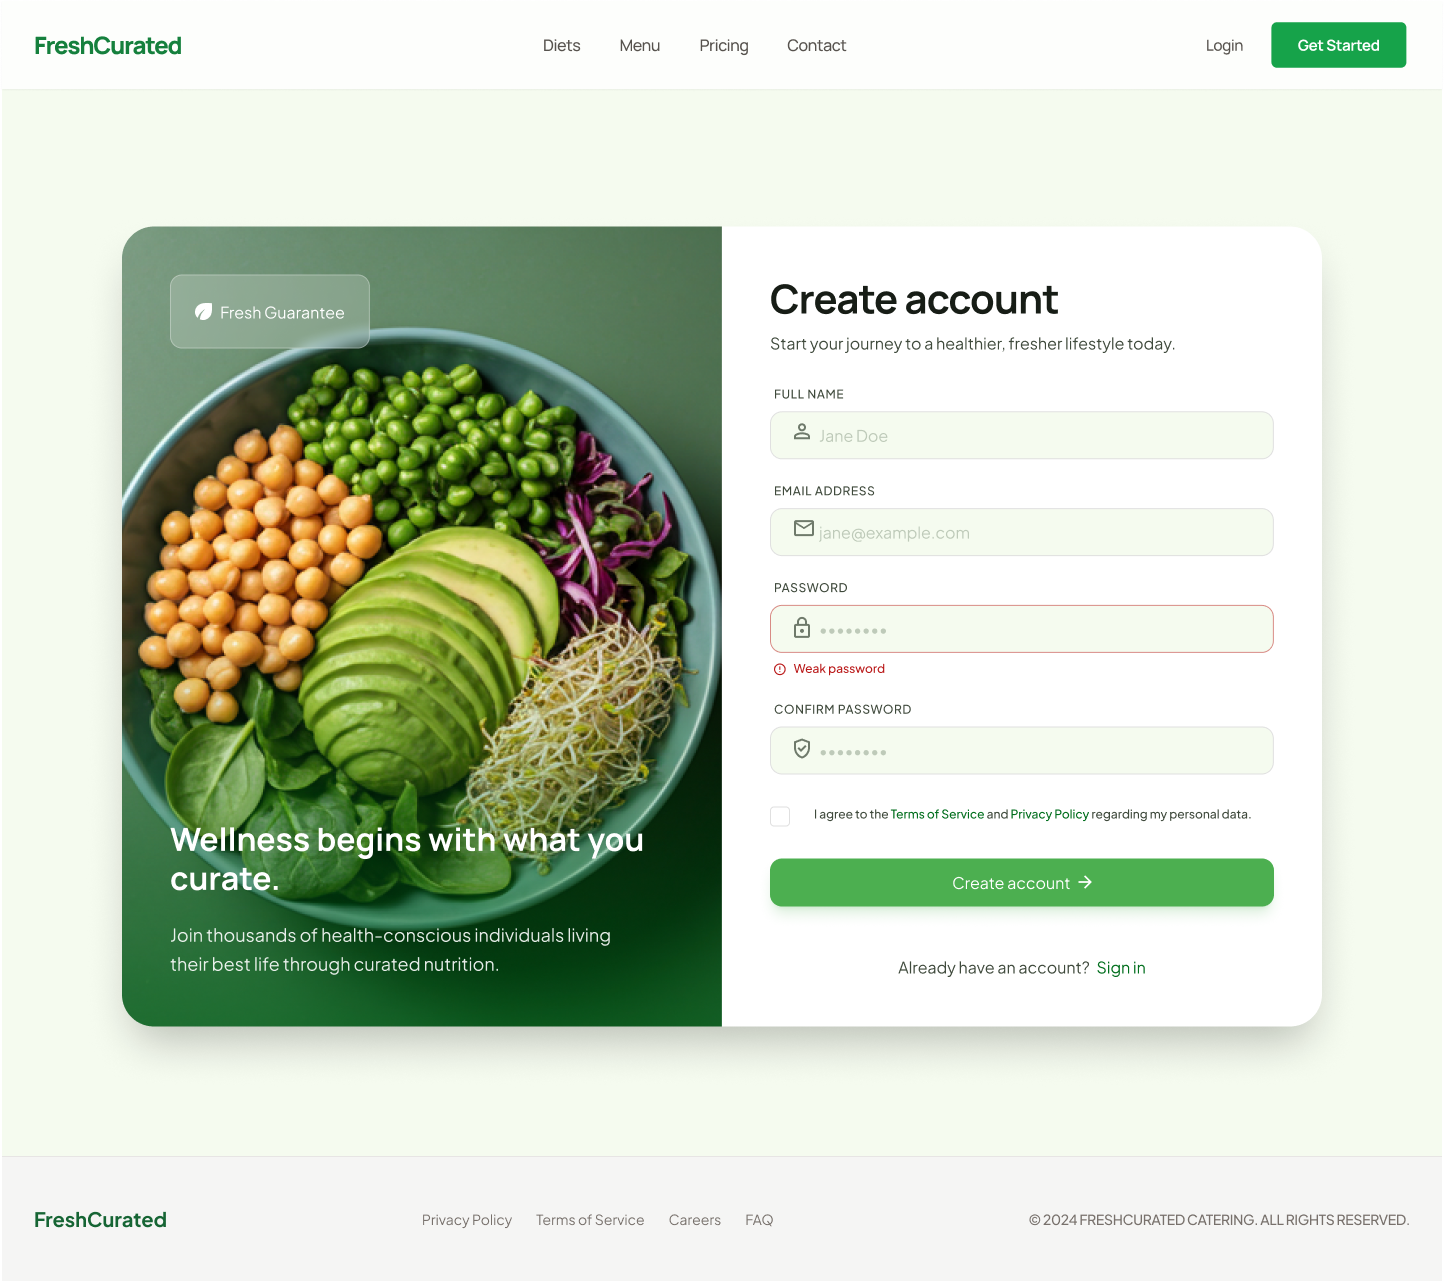
\includegraphics[width=0.6\textwidth]{figures/CreateAccount.png}
    \caption{Ekran tworzenia konta klienta}
    \label{fig:create_account}
\end{figure}

\begin{itemize}
    \item \textbf{Użytkownik niezalogowany}: Głównym celem jest zapoznanie się z ofertą dietetyczną. Funkcjonalności obejmują przeglądanie menu, weryfikację cenników oraz rozpoczęcie procesu składania zamówienia.
    \item \textbf{Użytkownik zalogowany}: Posiada pełny dostęp do personalizacji usług. Funkcjonalności obejmują dostęp do historii zamówień, zarządzanie kontem, edycję adresów dostaw oraz modyfikację parametrów aktywnych diet.
\end{itemize}

\section{Role administracyjne}
Zarządzanie działalnością cateringową podzielono na odrębne kompetencje, co znajduje odzwierciedlenie w strukturze panelu administratora przedstawionego na Rysunku \ref{fig:admin_panel_chapter2}.

\begin{figure}[ht]
    \centering
    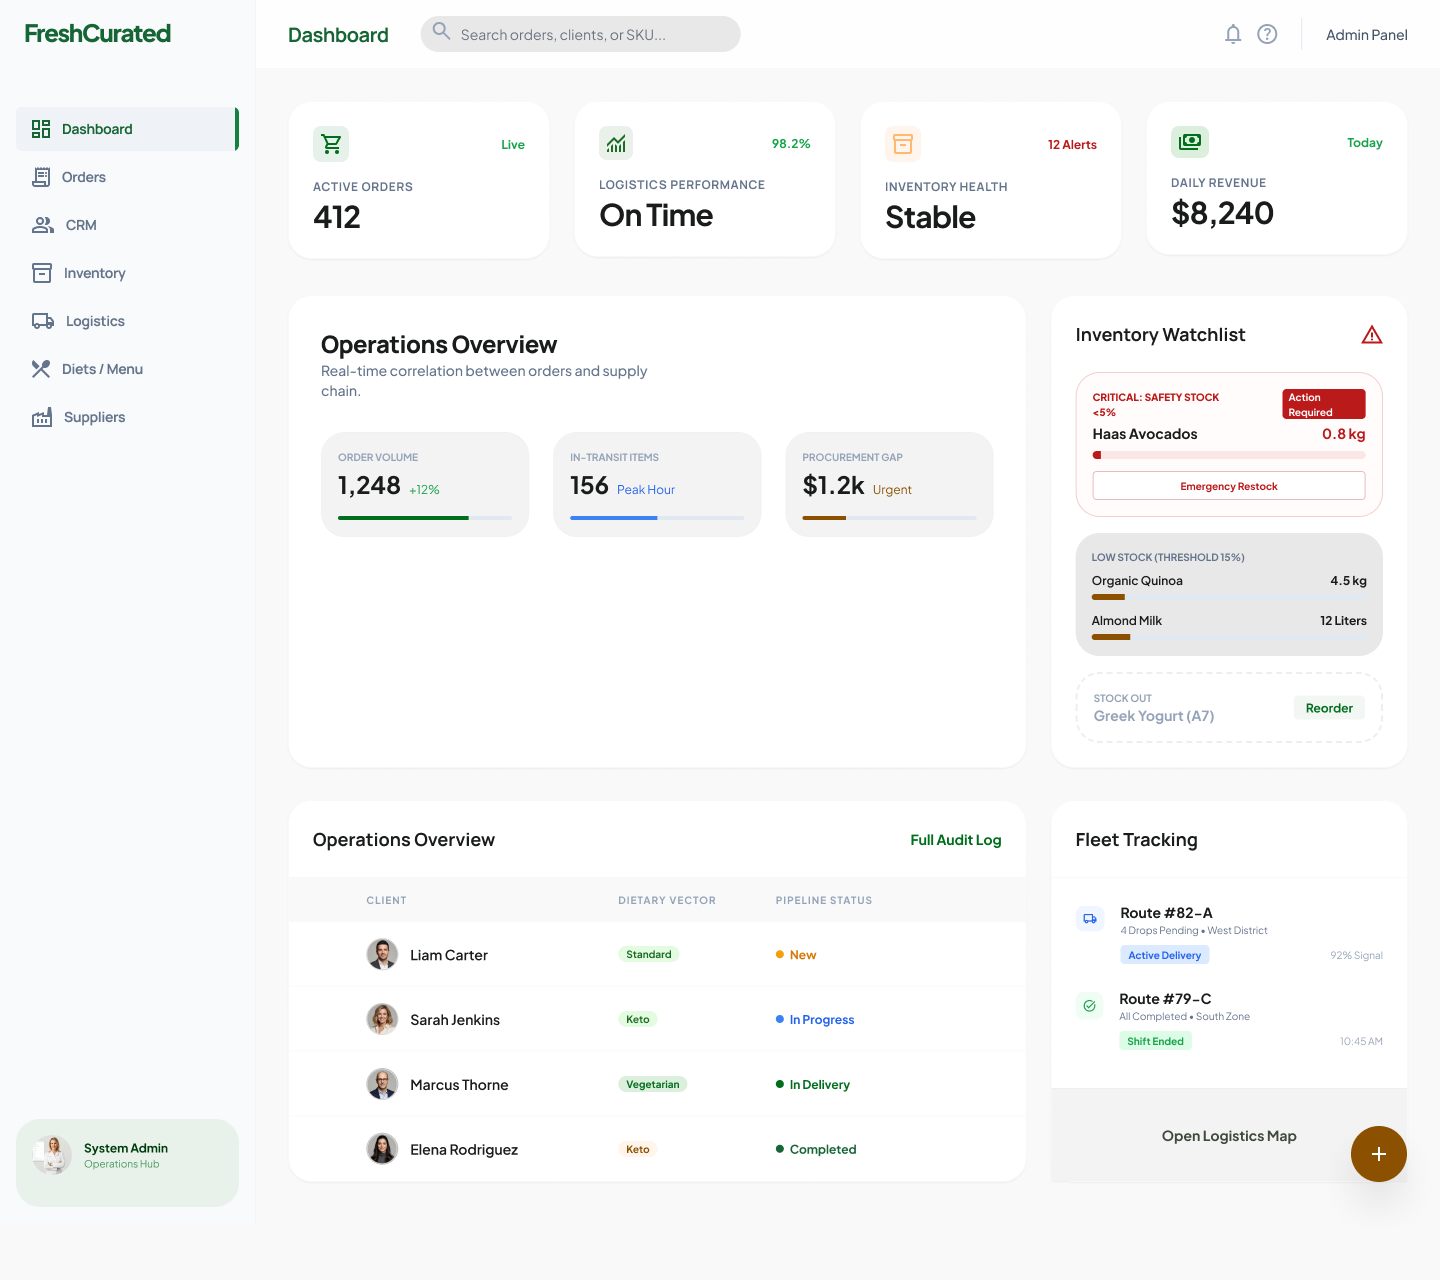
\includegraphics[width=0.8\textwidth]{figures/AdminPanel.png}
    \caption{Panel główny (Dashboard) administratora systemu}
    \label{fig:admin_panel_chapter2}
\end{figure}

Poniższa tabela przedstawia podział odpowiedzialności w zespole administracyjnym:

\begin{table}[ht]
    \centering
    \begin{tabular}{|l|p{8cm}|}
        \hline
        \textbf{Rola} & \textbf{Zakres odpowiedzialności} \\ \hline
        Administrator główny & Pełny dostęp do konfiguracji systemu i raportów. \\ \hline
        Pracownik biura & Bieżąca obsługa zamówień i relacji z klientami. \\ \hline
        Magazynier & Kontrola stanów składników i zarządzanie alertami braków. \\ \hline
        Logistyk/Kurier & Planowanie tras dostaw i nadzór nad realizacją. \\ \hline
    \end{tabular}
    \caption{Podział ról w panelu administracyjnym}
\end{table}

Taka architektura pozwala na bezpieczną separację obowiązków i zwiększa wydajność obsługi procesów biznesowych cateringu.
\chapter{Implementacja HTML i CSS}

\section{Zakres wdrożenia i responsywność}
Zgodnie z wymogami projektu, wybrane widoki zaprojektowane w programie Figma zostały zaimplementowane do działającego kodu przy użyciu technologii HTML5 oraz CSS3. 

Kluczowym założeniem podczas kodowania było zapewnienie pełnej responsywności (RWD - Responsive Web Design). Dzięki zastosowaniu nowoczesnych technik ostylowania (takich jak Flexbox oraz CSS Grid) a także zapytań medialnych (Media Queries), zaimplementowane interfejsy płynnie skalują się i dostosowują swój układ do szerokości okna przeglądarki. Potwierdza to, że system jest w pełni gotowy do obsługi zarówno na urządzeniach desktopowych, jak i mobilnych (smartfony, tablety).

Zgodnie z wymogiem prowadzącego, w procesie tworzenia bazowej struktury HTML oraz podstawowych reguł CSS wykorzystano wsparcie narzędzi AI (np. ChatGPT), przy czym wygenerowany kod został ręcznie zoptymalizowany, przetestowany i dostosowany do rygorystycznych wymogów responsywności.

\section{Struktura katalogów}
Aby zachować maksymalną czytelność i porządek w kodzie źródłowym, projekt został podzielony na logiczne foldery odpowiadające wdrożonym widokom. Poniżej przedstawiono strukturę katalogów zaimplementowanej części interfejsu:

\begin{itemize}
    \item \textbf{MainPage} -- Strona główna z ofertą.
    \begin{itemize}
        \item \texttt{MainPage.html} -- semantyczna struktura widoku
    \end{itemize}
    
    \item \textbf{Dashboard} -- Panel użytkownika z historią zamówień.
    \begin{itemize}
        \item \texttt{dashboard.html} -- struktura widoku panelu klienta
    \end{itemize}

    \item \textbf{OrderConfigurator} -- Zaawansowany konfigurator zamówienia.
    \begin{itemize}
        \item \texttt{configurator.html} -- struktura formularzy i kalendarza
        \item \texttt{style.css} -- style formularzy i siatki (Grid/Flexbox)
        \item \texttt{script.js} -- plik obsługujący interakcję (np. wybór dat)
    \end{itemize}

    \item \textbf{AdminDiets-menu} -- Moduł zarządzania dietami dla administratora.
    \begin{itemize}
        \item \texttt{Diets-menu-managment.html} -- struktura widoku panelu administracyjnego
    \end{itemize}
\end{itemize}

Takie podejście ułatwia ewentualną dalszą rozbudowę aplikacji oraz integrację front-endu z systemami back-endowymi.
\chapter{Szczegółowy opis funkcjonalności i modułów}

W tej części dokumentacji zaprezentowano szczegółowe zrzuty ekranu kluczowych modułów aplikacji, w tym ścieżki autoryzacji, zaawansowanych funkcji klienckich oraz zaplecza administracyjnego. Dla wybranych ekranów zestawiono widoki desktopowe i mobilne, co stanowi dowód na pełne dostosowanie interfejsu do urządzeń mobilnych (RWD).

\section{Ścieżka autoryzacji użytkownika}
Proces logowania i rejestracji został zaprojektowany z myślą o maksymalnej przejrzystości, budowaniu zaufania oraz minimalizacji czasu potrzebnego na założenie konta.

\begin{figure}[H]
    \centering
    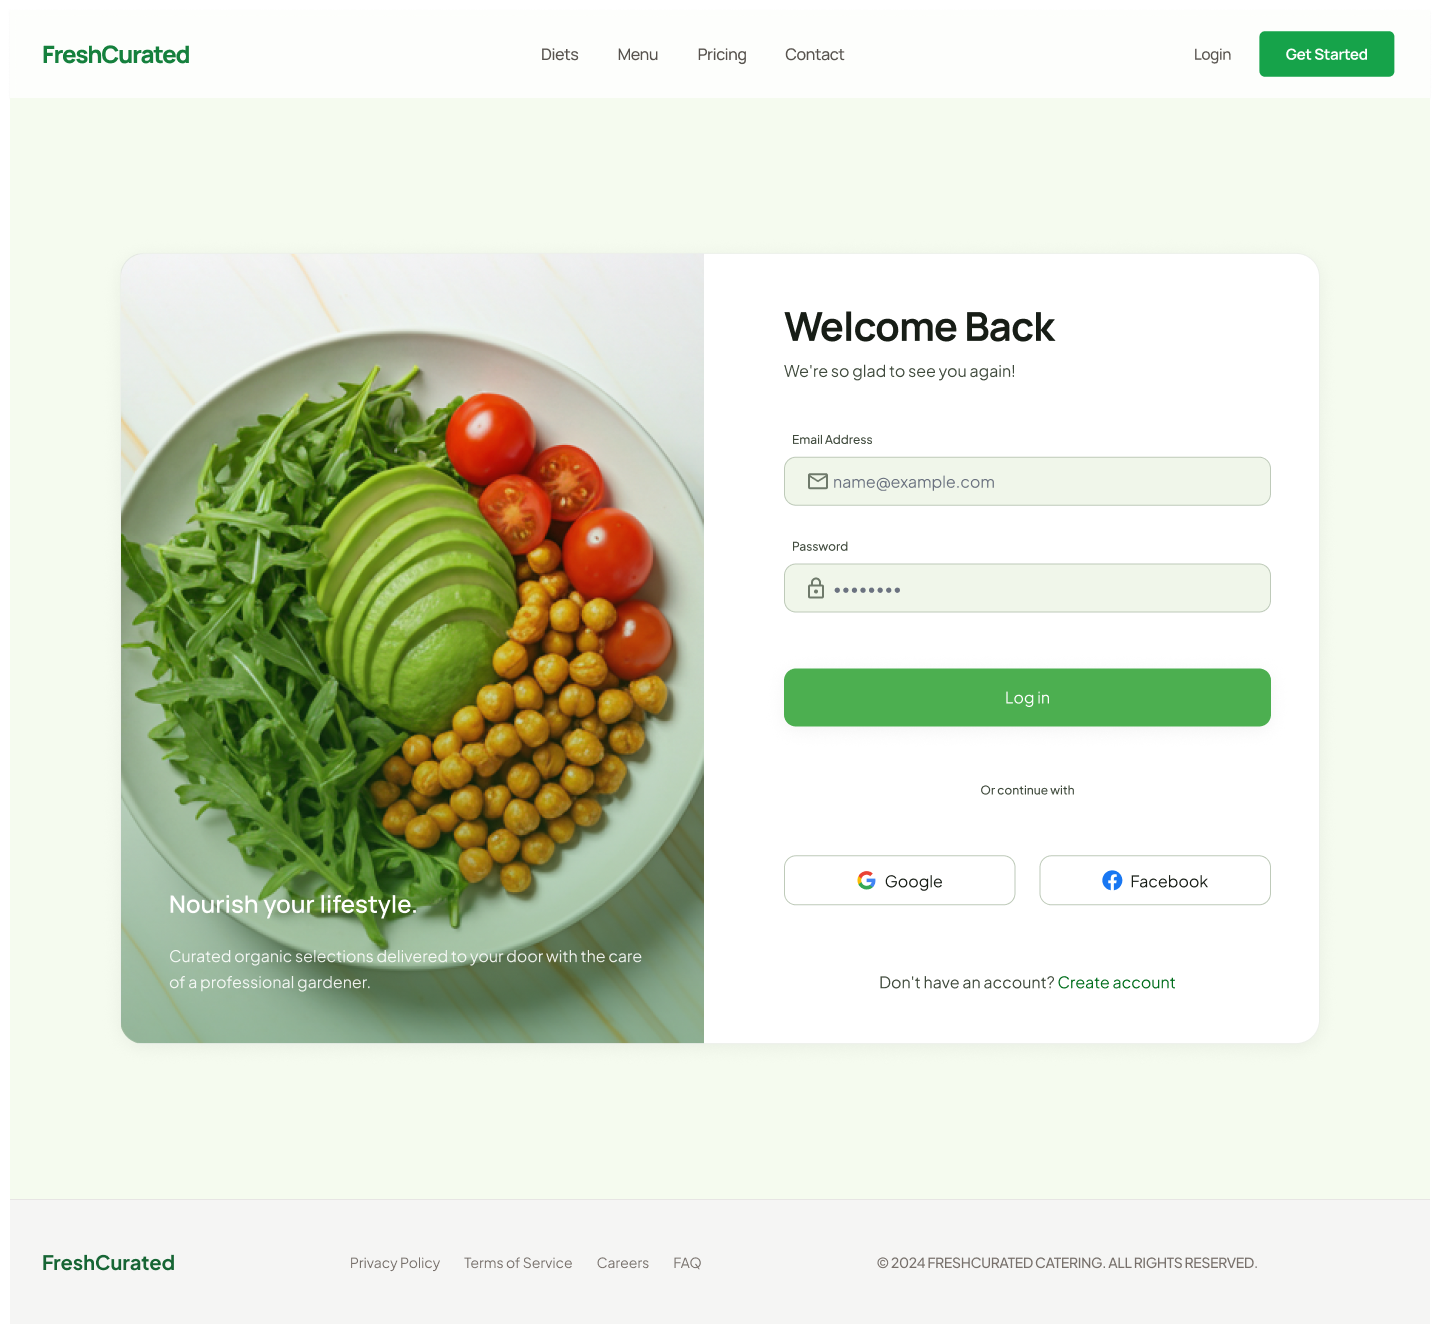
\includegraphics[height=7cm, keepaspectratio]{figures/WelcomeBackLogin.png}
    \hspace{0.5cm}
    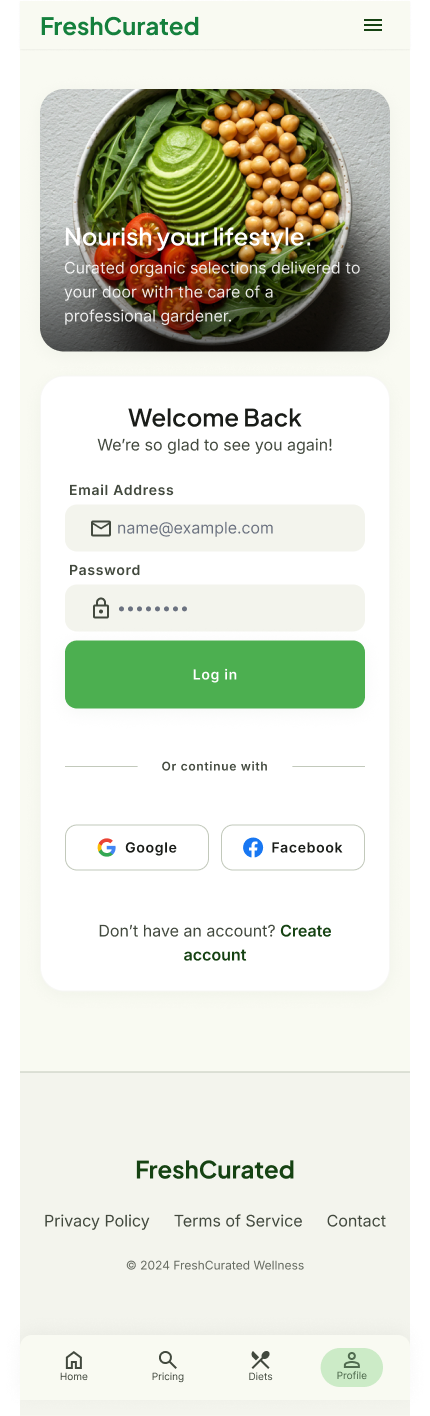
\includegraphics[height=7cm, keepaspectratio]{figures/WelcomeBackLogin-mobile.png}
    \caption{Ekran logowania (desktop i mobile) oferujący standardowe logowanie adresem e-mail oraz szybką integrację z platformami społecznościowymi.}
\end{figure}

Z kolei formularz rejestracji nowego konta posiada wbudowany mechanizm walidacji w czasie rzeczywistym, co znacznie poprawia użyteczność (UX).

\begin{figure}[H]
    \centering
    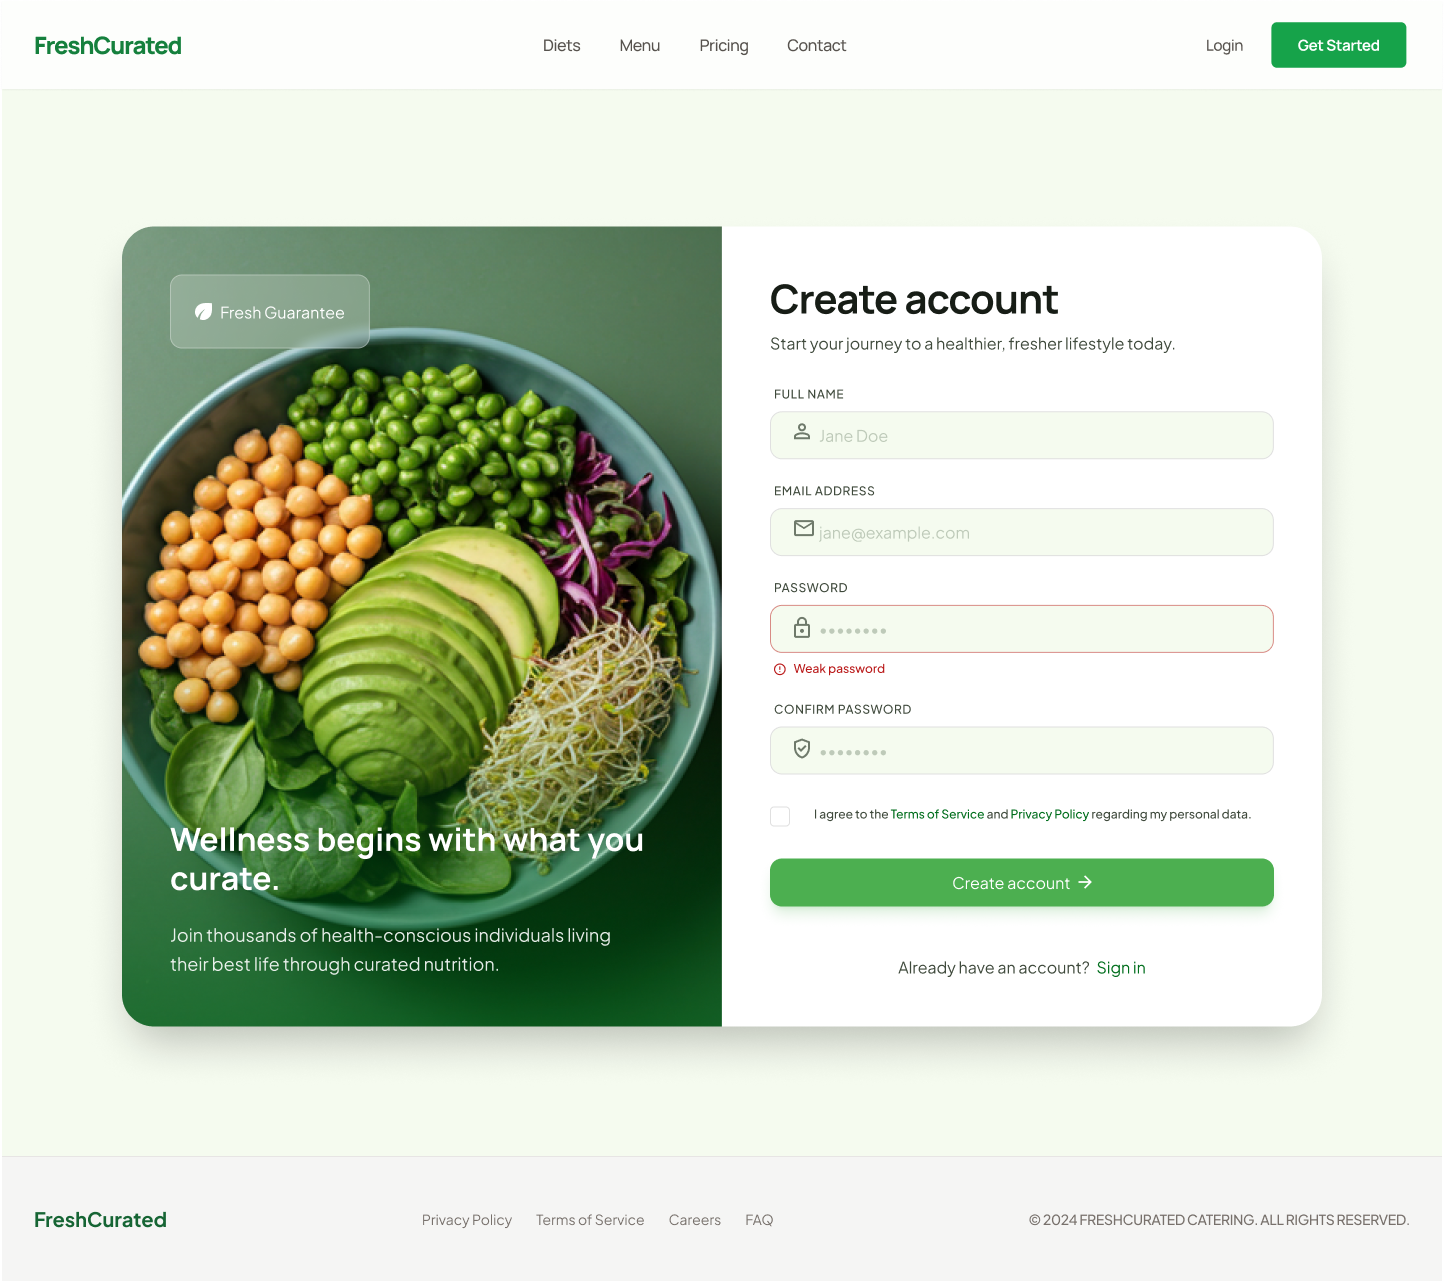
\includegraphics[height=7cm, keepaspectratio]{figures/CreateAccount.png}
    \hspace{0.5cm}
    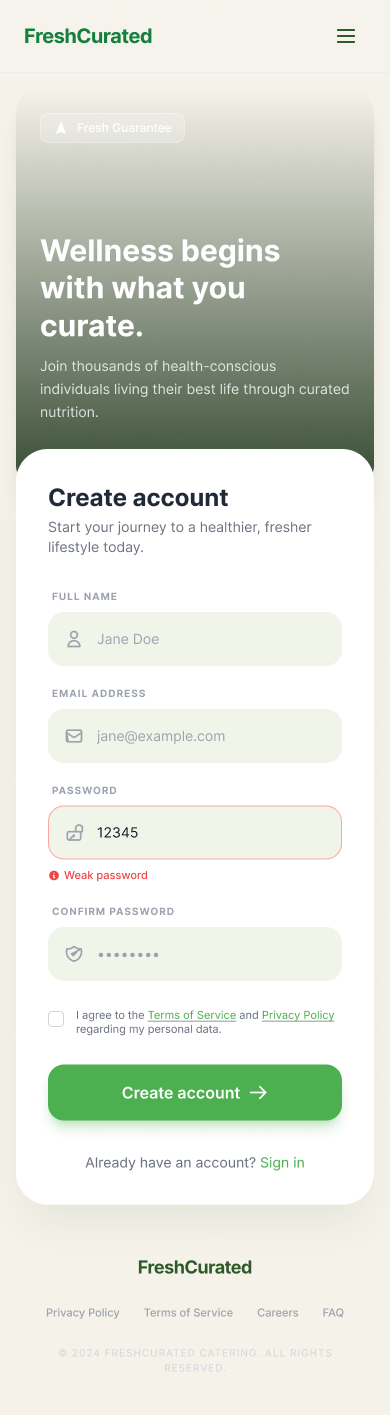
\includegraphics[height=7cm, keepaspectratio]{figures/CreateAccount-mobile.png}
    \caption{Formularz rejestracji z walidacją siły hasła.}
\end{figure}

\section{Rozszerzone funkcjonalności klienckie}
Aplikacja oferuje innowacyjne narzędzia wspierające klienta w świadomym wyborze optymalnego planu żywieniowego.

\begin{figure}[H]
    \centering
    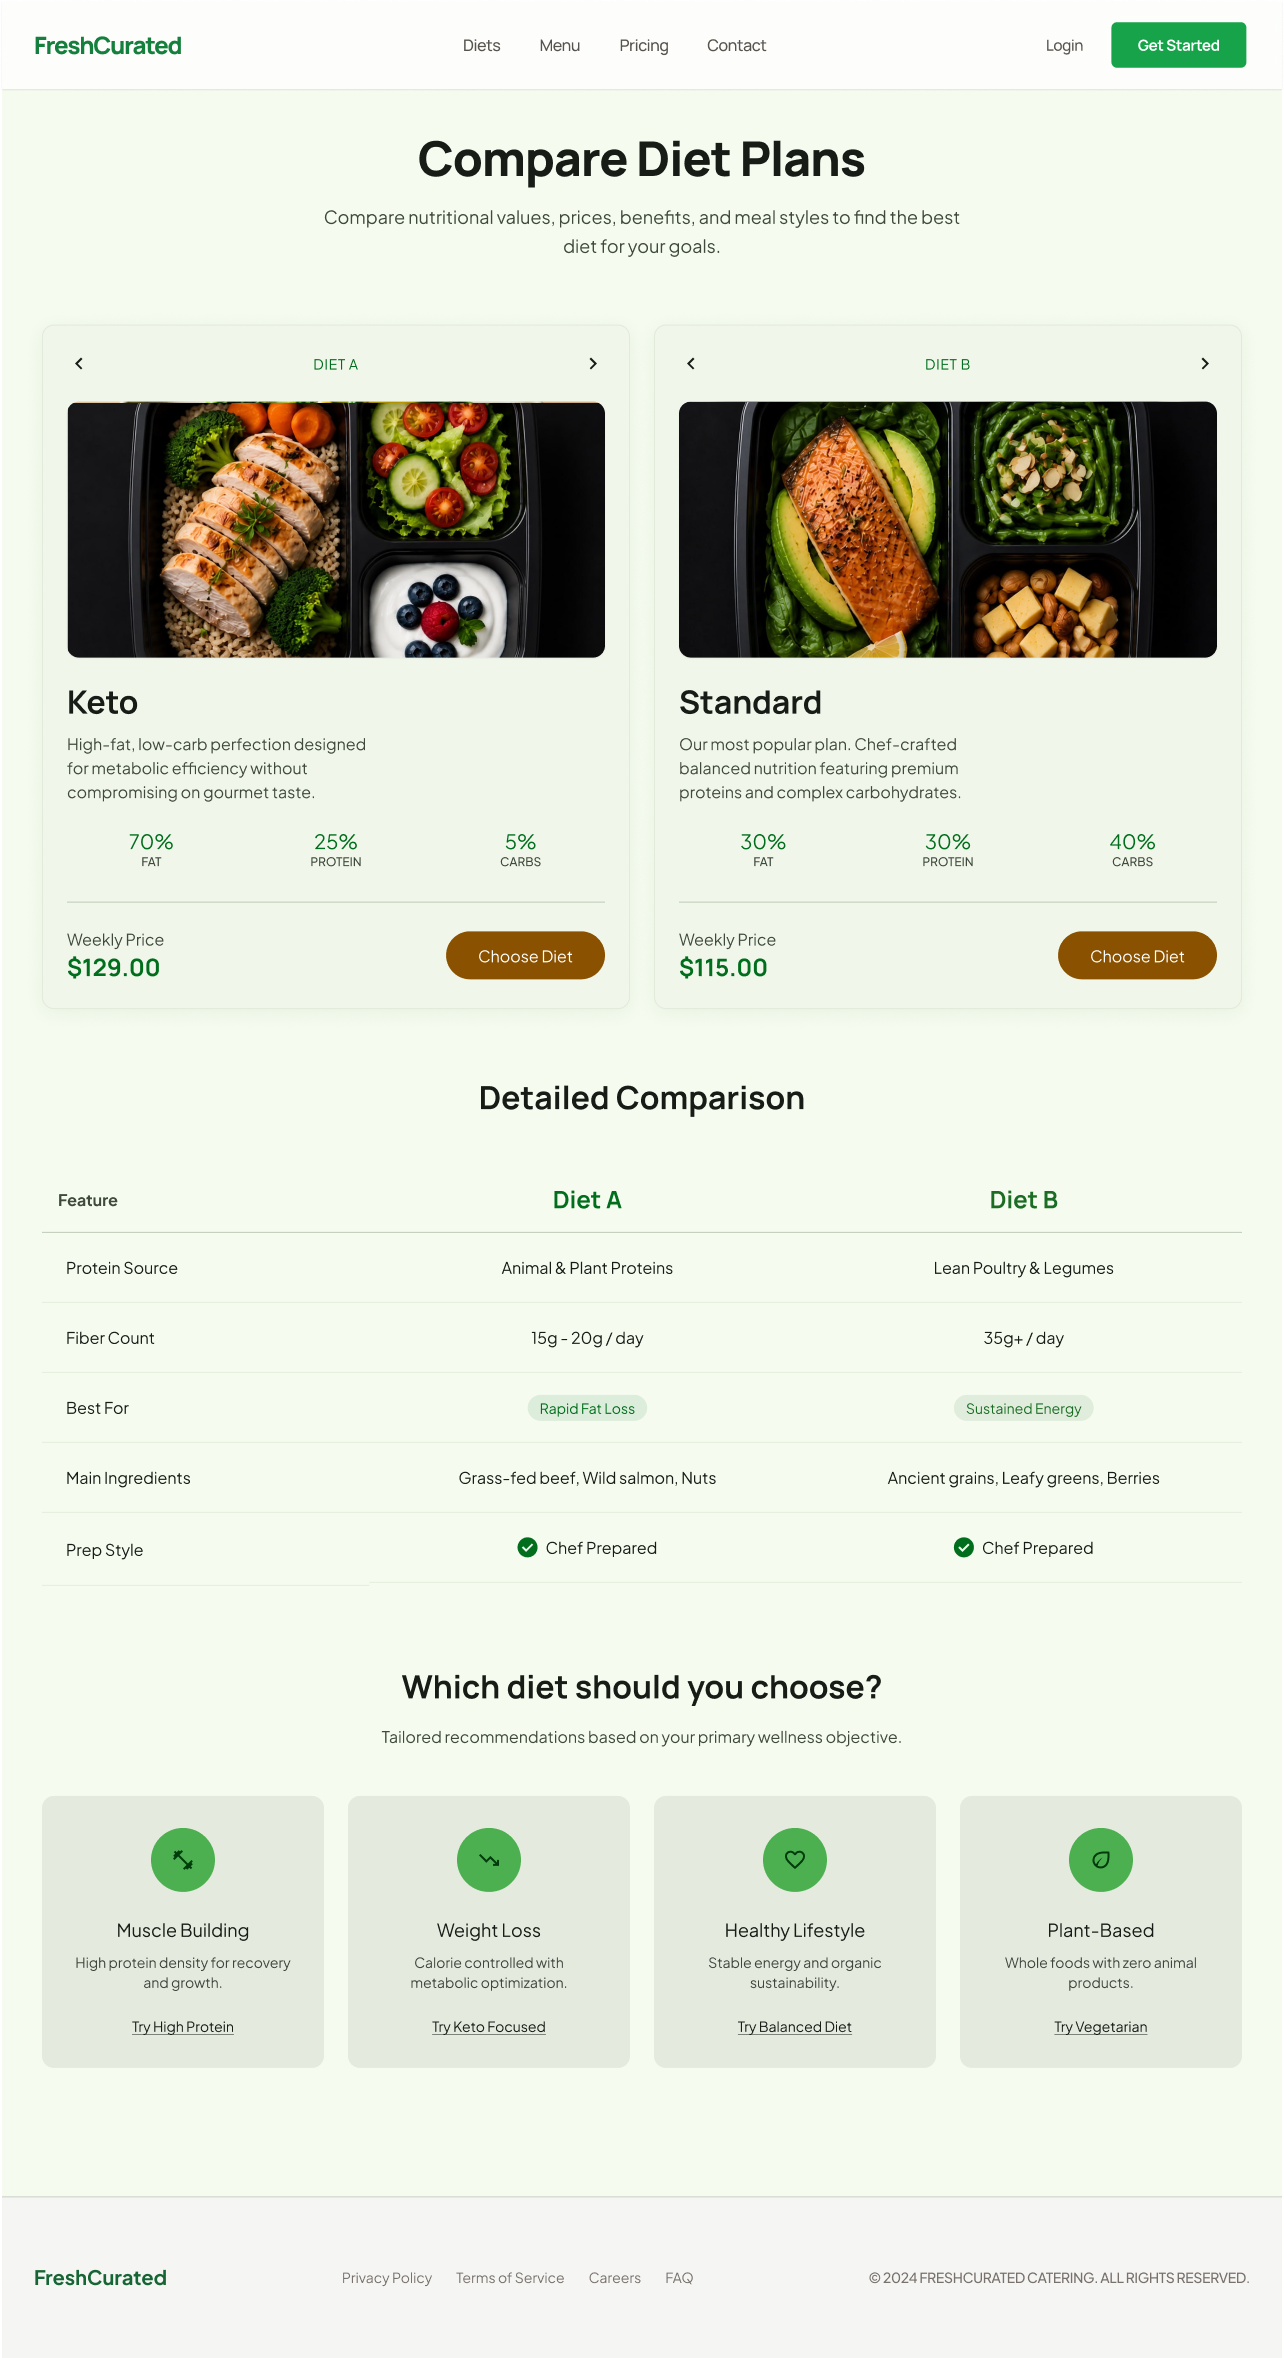
\includegraphics[height=8cm, keepaspectratio]{figures/CompareDiet.png}
    \hspace{0.5cm}
    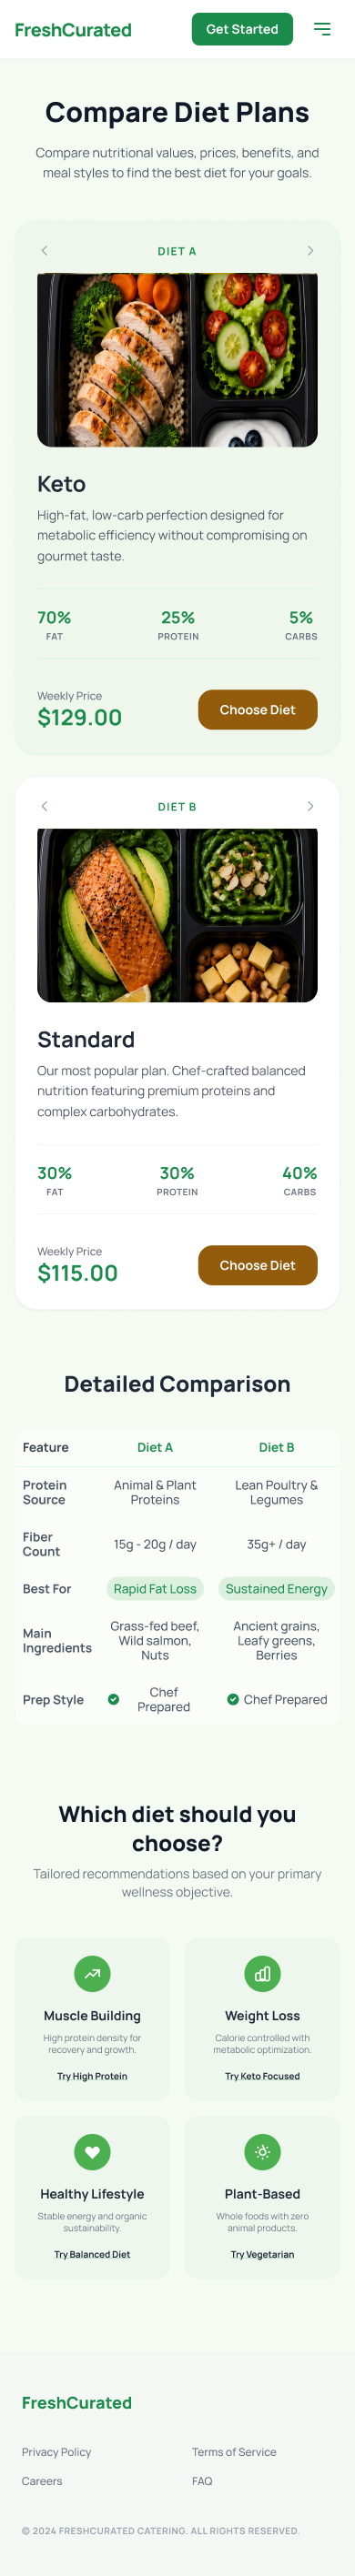
\includegraphics[height=8cm, keepaspectratio]{figures/CompareDiet-mobile.png}
    \caption{Moduł porównywarki diet (desktop i mobile). Pozwala na bezpośrednie zestawienie dwóch planów i ich makroskładników.}
\end{figure}

\section{Moduły administracyjne: Logistyka i Magazyn}
Sprawne działanie firmy cateringowej wymaga zaawansowanych narzędzi dla pracowników zaplecza. Moduły te agregują najważniejsze dane operacyjne.

\begin{figure}[H]
    \centering
    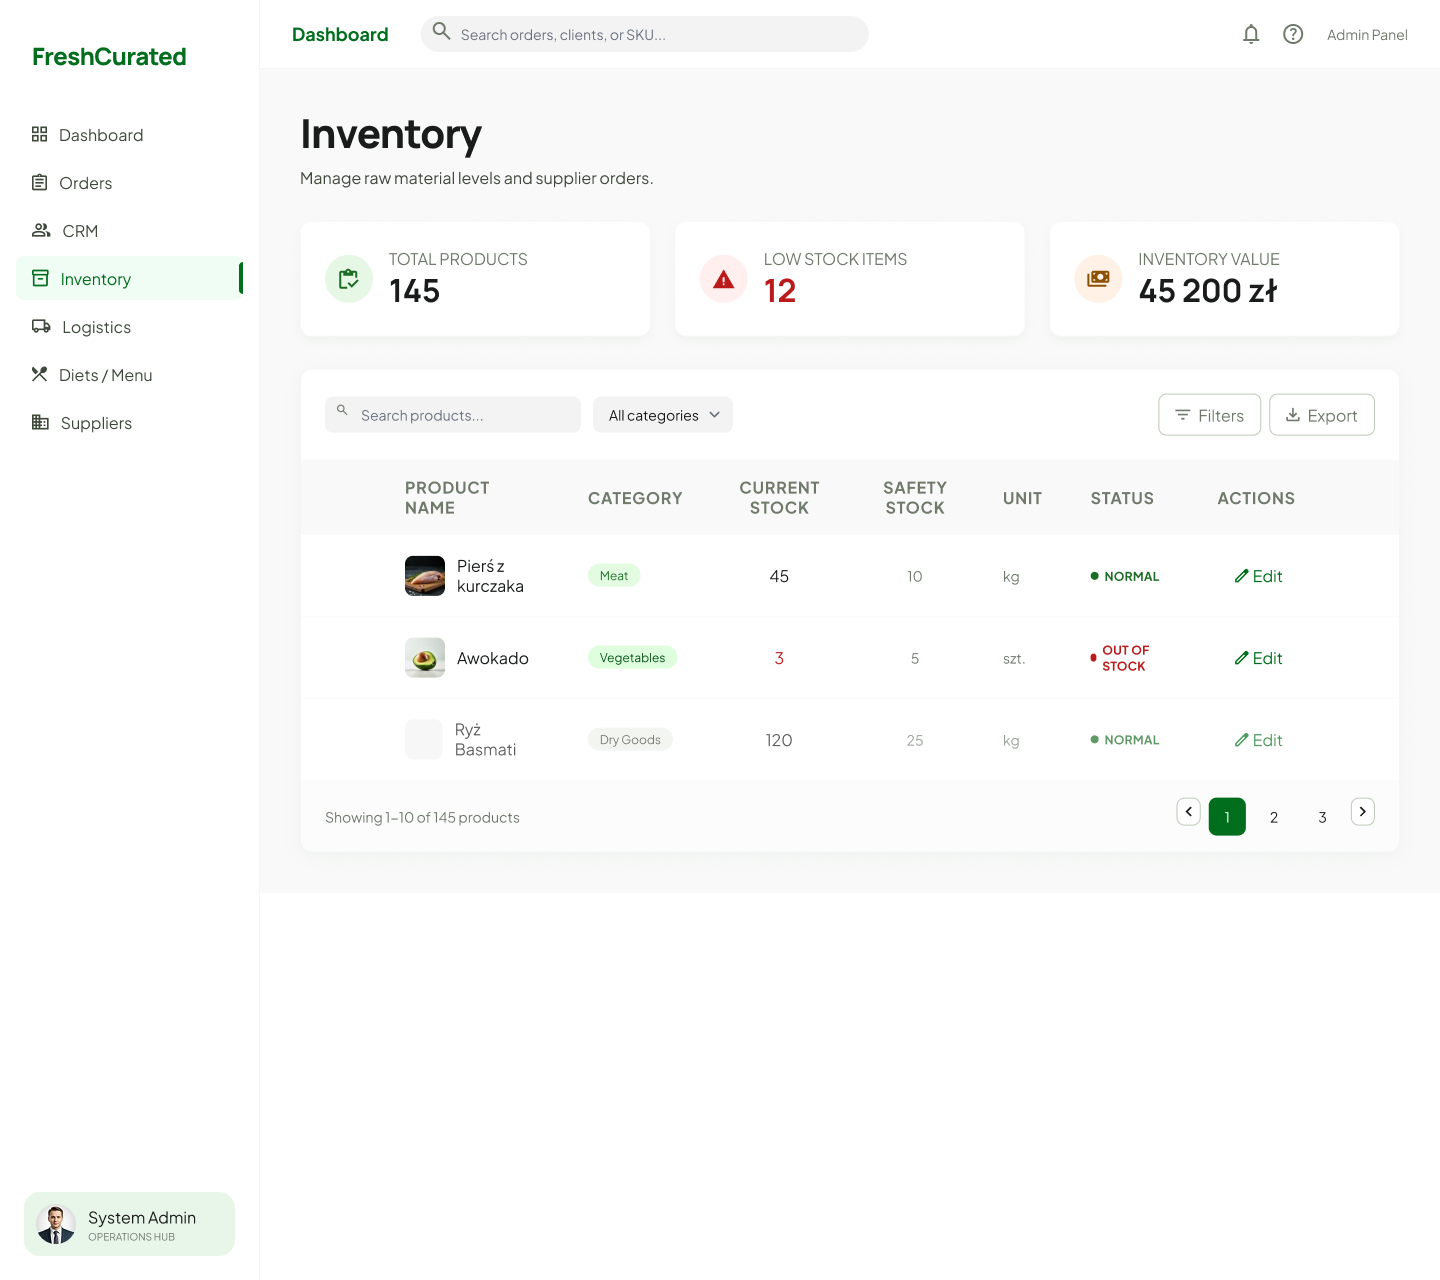
\includegraphics[width=0.85\textwidth, height=8.5cm, keepaspectratio]{figures/admin-inventory.png}
    \caption{Panel zarządzania magazynem (Inventory) z widocznym systemem ostrzegania o niskich stanach magazynowych.}
\end{figure}

Kolejnym kluczowym elementem jest główny panel logistyczny ułatwiający zarządzanie kurierami oraz monitorowanie statusów dostaw na bieżąco.

\begin{figure}[H]
    \centering
    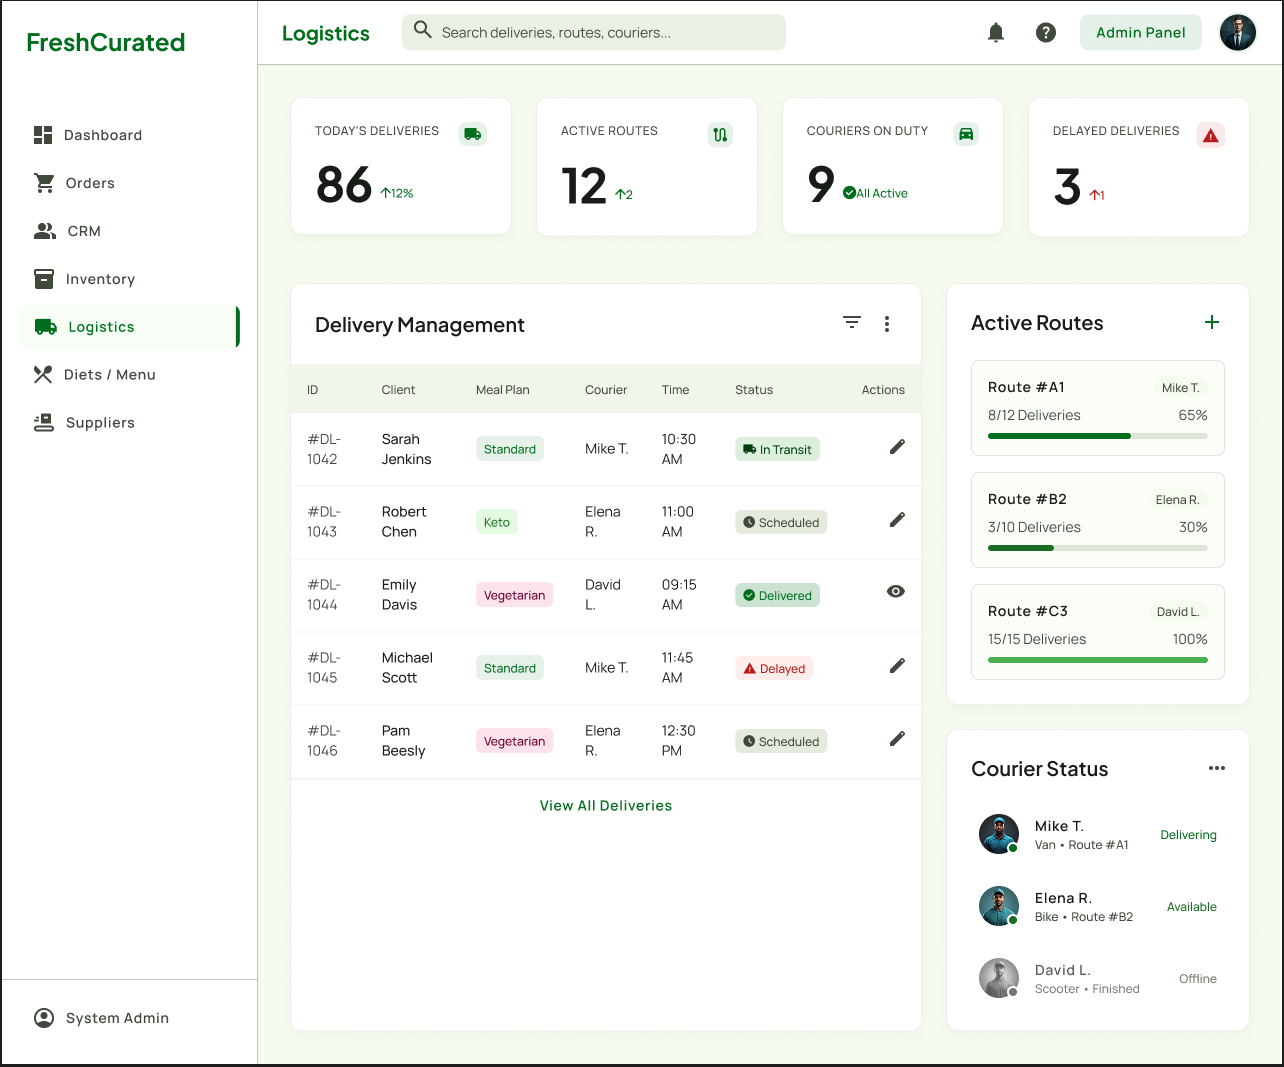
\includegraphics[width=0.85\textwidth, height=8.5cm, keepaspectratio]{figures/admin-logistic.png}
    \caption{Główny panel logistyczny ułatwiający zarządzanie kurierami i trasami.}
\end{figure}

Wsparcie dla logistyki stanowi również interaktywny podgląd na żywo, który ułatwia optymalizację łańcucha dostaw firmy.

\begin{figure}[H]
    \centering
    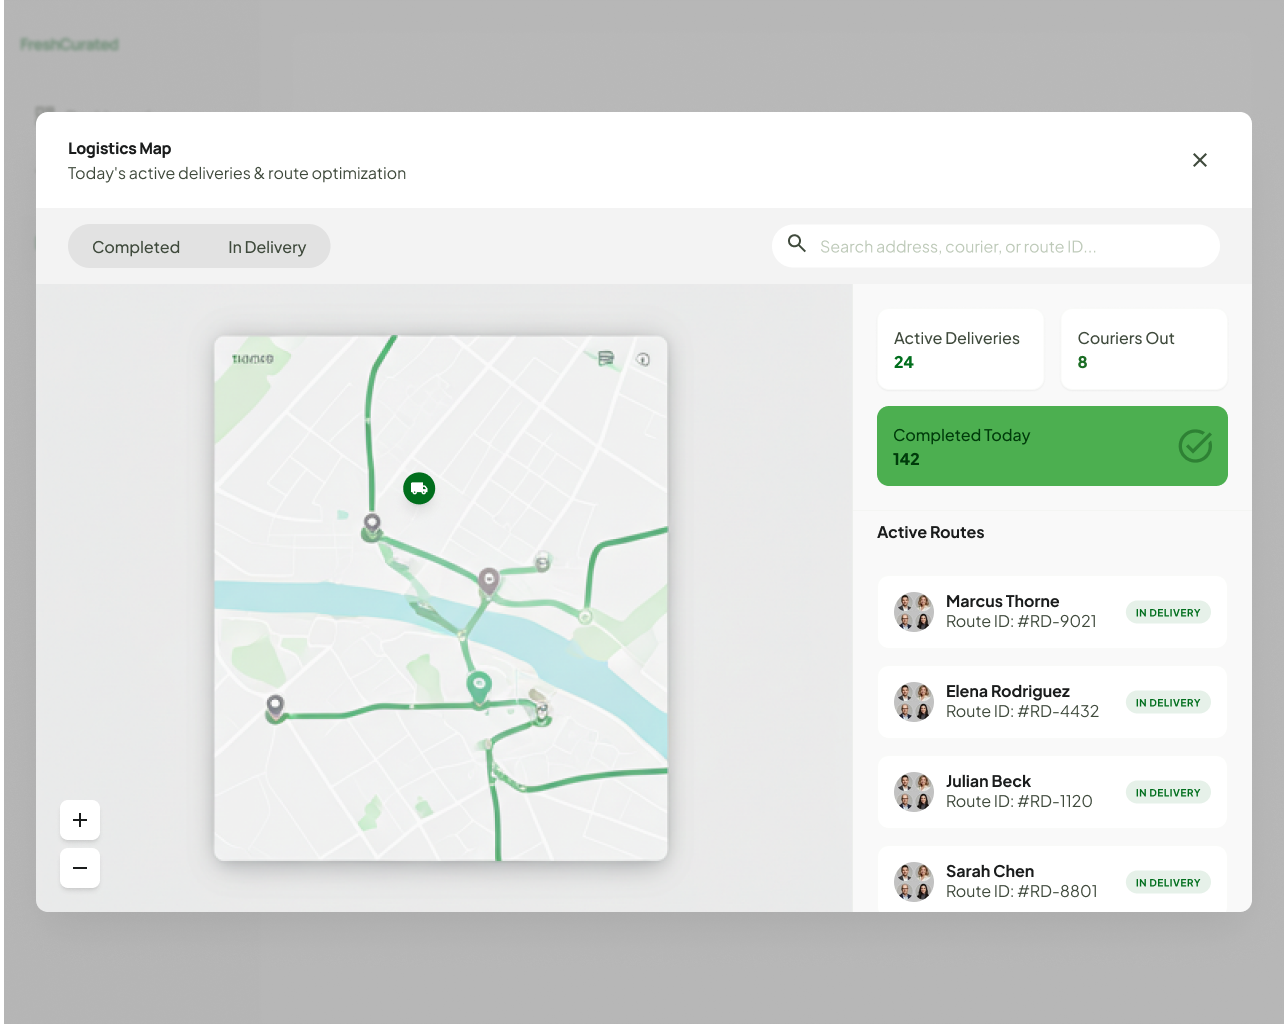
\includegraphics[height=7cm, keepaspectratio]{figures/ModalMap.png}
    \hspace{0.5cm}
    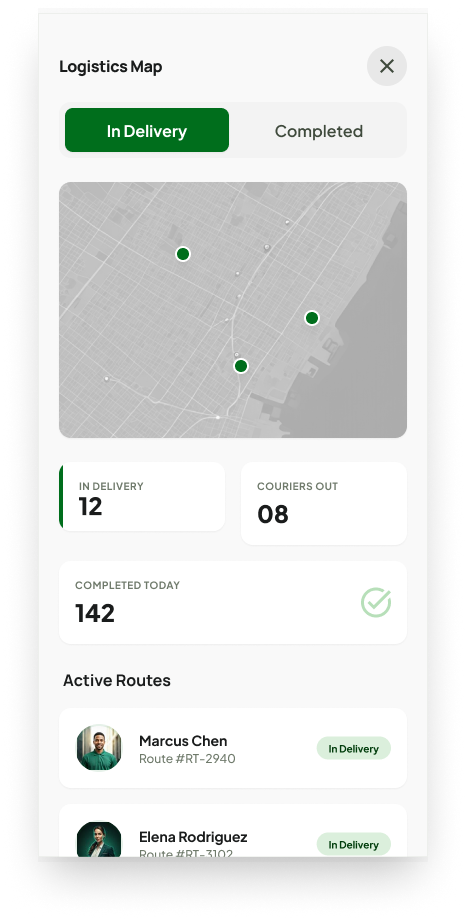
\includegraphics[height=7cm, keepaspectratio]{figures/ModalMap-mobile.png}
    \caption{Interaktywna mapa logistyczna przedstawiająca aktywne trasy kurierów i punkty dostaw.}
\end{figure}
\chapter{Organizacja pracy i wykorzystanie AI}
Zgodnie z wymaganiami projektu, dokumentujemy wykorzystanie narzędzi sztucznej inteligencji. Narzędzia AI (np. ChatGPT, Midjourney) zostały wykorzystane wyłącznie w celach pomocniczych, takich jak generowanie przykładowych tekstów (tzw. fillerów) do makiet oraz tworzenie grafik posiłków do interfejsu. Całość architektury informacji, ścieżki UX oraz design UI zostały opracowane samodzielnie przez zespół.
\chapter{Podsumowanie}
Projekt interfejsu kompleksowo wspiera zarządzanie cateringiem dietetycznym. Zaprezentowane warianty widoków, od ekranów zakupowych po skomplikowany panel logistyczno-magazynowy, udowadniają wysoką złożoność aplikacji. Dzięki intuicyjnej nawigacji i zintegrowanym funkcjom biznesowym aplikacja realizuje zadania automatyzacji procesów oraz łatwego zamawiania.

% --- < spisy > ---
\clearpage
\addcontentsline{toc}{section}{\textbf{Spis rysunków}}
\listoffigures
\clearpage

%\addcontentsline{toc}{section}{\textbf{Spis tabel}}
%\listoftables
%\clearpage

\addcontentsline{toc}{section}{\textbf{Spis listingów}}
\lstlistoflistings
\clearpage

% --- < aneksy > ---
\chapter*{Aneks A: Oświadczenie autorów projektu}
\addcontentsline{toc}{section}{Aneks A: Oświadczenie autorów projektu}

Jako autorzy niniejszego projektu zaliczeniowego oświadczamy, że praca została wykonana przez nas samodzielnie, a zaprojektowane widoki interfejsu są wynikiem pracy naszego zespołu.

\vspace{0.5cm}
\noindent\textbf{Oświadczenie dotyczące wykorzystania narzędzi AI:} \\
Zgodnie z wytycznymi prowadzącego, pragniemy doprecyzować rolę narzędzi opartych na sztucznej inteligencji w naszym projekcie:

\begin{itemize}
    \item Narzędzia AI (ChatGPT) \textbf{zostały wykorzystane} w projekcie wyłącznie w charakterze asystenta – do wygenerowania przykładowych tekstów (tzw. placeholderów/fillerów) na widokach oraz stworzenia grafik potraw i zdjęć profilowych użytych w makietach.
    % UWAGA: Jeśli w ogóle nie użyliście AI do żadnego obrazka ani tekstu, usuń powyższy punkt i zostaw tylko ten poniżej:
    % \item Narzędzia AI \textbf{nie zostały wykorzystane} na żadnym etapie prac nad projektem.
\end{itemize}

Oświadczamy, że cała architektura informacji, układ poszczególnych widoków, ścieżki użytkownika (UX) oraz styl wizualny (UI) zostały zaprojektowane przez nas w pełni samodzielnie.

\vspace{1.5cm}
\begin{flushright}
\begin{tabular}{c}
....................................................... \\
Yevhen Marchak \\[0.5cm]
....................................................... \\
Mykhailo Kleban \\[0.5cm]
....................................................... \\
Damian Kania \\[0.5cm]
....................................................... \\
Mikołaj Kopacz \\[0.5cm]
....................................................... \\
Artur Jurkowski \\
\end{tabular}
\end{flushright}

\end{document}
